\documentclass{beamer}
\usetheme{Boadilla}

\usepackage[english]{babel}
\usepackage[T1]{fontenc}
\usepackage[latin1]{inputenc}
\usepackage{tikz}
\usepackage{verbatim}
\usepackage{animate}
\usepackage{calc}
\usepackage{fp}
\usepackage{times}

\title[MUMmer]{Alignment of whole genomes using MUMmer}

\subtitle{Presentation in Algorithms in Bioinformatics (T�111F autumn 2014)}

\author{Hannes P�tur Eggertsson}

\date{November 18, 2014}

%\setbeamertemplate{frametitle}[default][center]


\begin{document}

\begin{frame}[plain]
\titlepage
\end{frame}

%%%%%%%%%%%%%%%%%%%%%%%%%%%%%%%%%%%%%%%%%%%%%%%%%%%%%%%%%%%%%%%%

\begin{frame}{Motivation}
Let's go back to 1999... (some things that will remind you of that wonderful time)

{
	
\includegraphics[width=0.3\textwidth]{img/Win98.png}<2-4>
	
\includegraphics[width=0.35\textwidth]{img/blue.png}<3-4>
	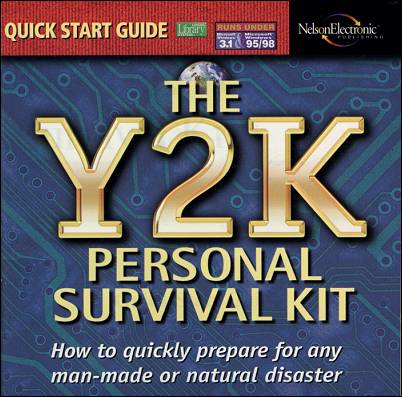
\includegraphics[width=0.34\textwidth]{img/y2k.jpg}<4>
}
\end{frame}

\begin{frame}{Motivation}
In 1999...
\begin{itemize}
\item The number of sequenced genomes was very low but increasing rapidly
\item When a new genome is sequenced, one could ask himself:
\begin{itemize}
\item How does this genome align to the other genomes?
\end{itemize}
\end{itemize}

Problem: 
\begin{itemize}
\item We had algorithms that were used for single gene sequences (up to 10,000 bp)
\item But, they won't work well with whole genomes (can be millions of base pairs or more).
\item On the other algorithms they'd either
\begin{itemize}
\item Take up way too much memory or
\item Have unacceptable computational time
\end{itemize}
\end{itemize}
\end{frame}

\begin{frame}{Problem description}
\begin{itemize}
\item[In] Two genomes, A and B. Both could be very large (possibly over 1 Mbp)

{
	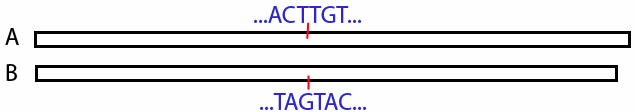
\includegraphics[width=0.85\textwidth]{img/genomeBefore.png}
}

\item[Out] Align the two genomes using insertions and deletions (or for short, indels) to maximize the matches.

{
	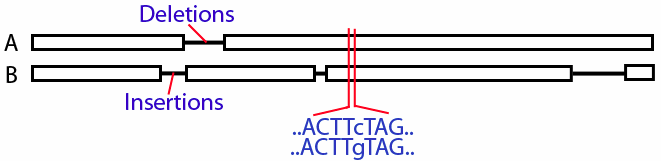
\includegraphics[width=0.85\textwidth]{img/genomeAfter.png}
}
\end{itemize}
\end{frame}

\begin{frame}{Introduction to MUMmer}
%	{ 
%		\includegraphics[width=0.6\textwidth]{img/turmite.png}
%	}
MUMmer:
\begin{itemize}
\item Was published in 1999.
\item Is a system used to align whole genome sequences.
\item Uses suffix trees as a data structure.
\item Tries to find large unique chunks of exact matches on both genomes.
\begin{itemize}
\item So it will only work well for two genomes that are similar/related.
\end{itemize}
\item Has been open-source since 2004 (when MUMmer 3 was released).
\item Doesn't guarantee the optimal solution, just a good one.
\item The algorithm can be split into several steps.
\end{itemize}
\end{frame}

\begin{frame}{Step 1: Creating a suffix tree}
A suffix tree is a compact representation that stores all possible suffixes of an input sequence.
\begin{itemize}
\item Square nodes are leaves.
\begin{itemize}
\item Store information about the starting position of the suffix.
\end{itemize} 
\item Circular nodes are internal nodes.
\begin{itemize}
\item That means two or more sequences share the same prefix.
\item Store information about the length of the shared prefix.
\end{itemize}
\end{itemize}
\begin{center}
	{
		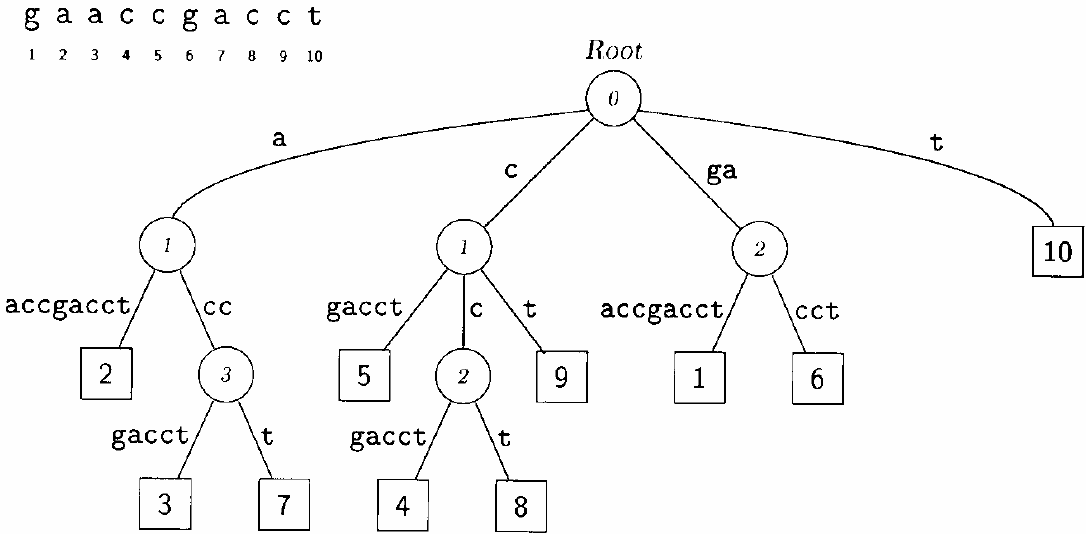
\includegraphics[width=0.65\textwidth]{img/suffixTree.png}
	}
\end{center}
Creating a suffix tree takes $O(n)$ time and space.
\end{frame}

\begin{frame}{Step 2: MUM decomposition}
Let us first define what a MUM is
\begin{definition}
A subsequence is a MUM (Maximal Unique Matches) if and only if:
\begin{itemize}
\item The subsequence has an exact match on both genomes
\item It is not a subsequence of another matched sequence
\begin{itemize}
\item This means the sequence is surrounded be mismatches
\end{itemize}
\item It is unique
\begin{itemize}
\item It appears exactly once in both genomes
\end{itemize}
\item Almost always uses some minimum sequence length.
\end{itemize}
\end{definition}
\begin{example}
\texttt{tcgatcGACGATCGCGGCCGTAGATCGAATAACGAGAGAGCATAAcgactta}
\texttt{gcattaGACGATCGCGGCCGTAGATCGAATAACGAGAGAGCATAAtccagag}
\end{example}
We can find these MUMs using the suffix tree (further details later).
\end{frame}

\begin{frame}{Step 3: Sorting the matches found in the MUM alignment}
Once we have found the MUMs, we enumerate them like this:

\vspace{0.2cm}{
	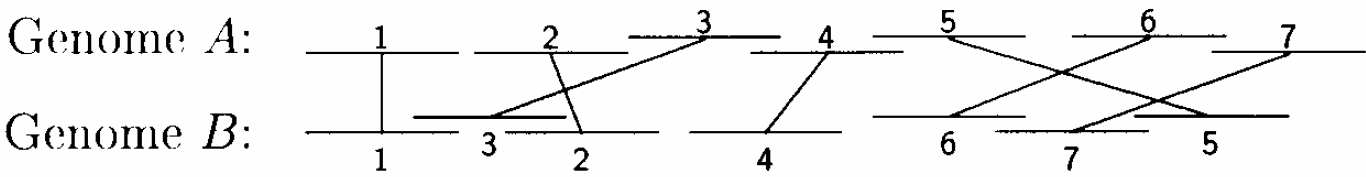
\includegraphics[width=0.75\textwidth]{img/sort1.png}
}\vspace{0.2cm}

\textbf{Problem:} We cannot align all MUMs because they aren't in the same order in both genomes.

\textbf{Solution:} Align as many MUMs as we can:
\begin{itemize}
\item We find the longest increasing sequence for genome B.
\begin{itemize}
\item In this case the sequence is <1,3,2,4,6,7,5>.
\end{itemize}
\item We can do this in $O(K \log K)$ time, where $K$ is the number of MUMs. Since in general $K << N/\log N$ this step takes $O(n)$ time.
\end{itemize}

\vspace{0.2cm}{
	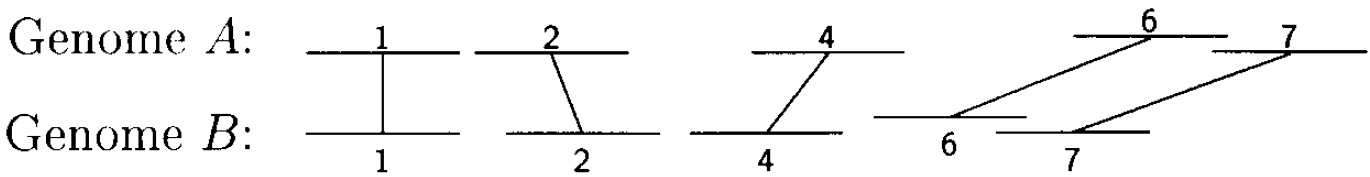
\includegraphics[width=0.75\textwidth]{img/sort2.png}
}
\end{frame}

\begin{frame}{Step 4: Closing the gaps}
Everything in between the MUMs is called \textbf{gaps}.
\begin{itemize}
\item To find alignment for the gaps we use any alignment algorithm.
\item The first version of MUMmer uses the Smith-Waterman alignment algorithm (which takes $O(n^2)$ time).
\item If the gaps are too large for the alignment algorithm we need to recursively find new MUMs in that region using a smaller minimum sequence length than before.
\end{itemize}

\end{frame}

\begin{frame}{Step 5: Output results}
The final alignment is the alignment of MUMs and gaps combined.
\begin{itemize}
\item If the two genomes are very similar, then the MUMs sequences will...:
\begin{itemize}
\item ...be long.
\item ...cover most of the genome.
\item ...rarely be a random match. Therefore few or no errors.
\item ...make the algorithm run fast (almost linear time)
\end{itemize}
\item If the genomes are very different, then the MUMs sequences will...:
\begin{itemize}
\item ...be short.
\item ...cover a small part of the genome.
\item ...often be a random match. Therefore many errors.
\item ...make the algorithm run slow.
\end{itemize}
\end{itemize}

\end{frame}

\begin{frame}{Creating a suffix tree}
\only<1>{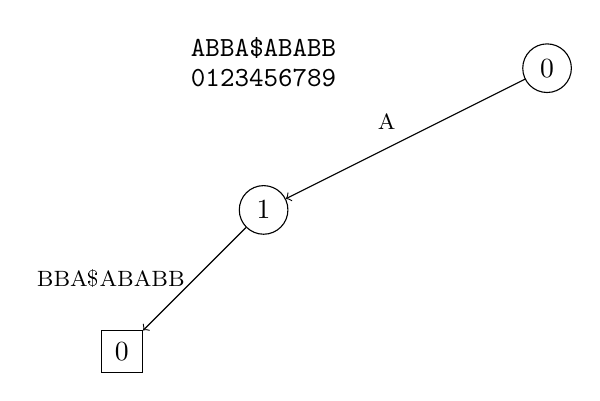
\begin{tikzpicture}[scale=1.8]
\draw (-2,0) node[above] {\texttt{\textbf{ABBA\$ABABB}}};
\draw (-2,-0.2) node[above] {\texttt{0123456789}};
\path (0,0) node[circle,minimum size=15pt,draw] (00) {0};

\path (-2,-1) node[circle,minimum size=15pt,draw] (A){1};
\draw[->] (00) -- node[above left]{\footnotesize A} (A);
\path (-3,-2) node[rectangle,minimum size=15pt,draw] (AB){0};
\draw[->] (A) -- node[left]{\footnotesize BBA\$ABABB} (AB);
\end{tikzpicture}}

\only<2>{\hspace*{-0.25cm}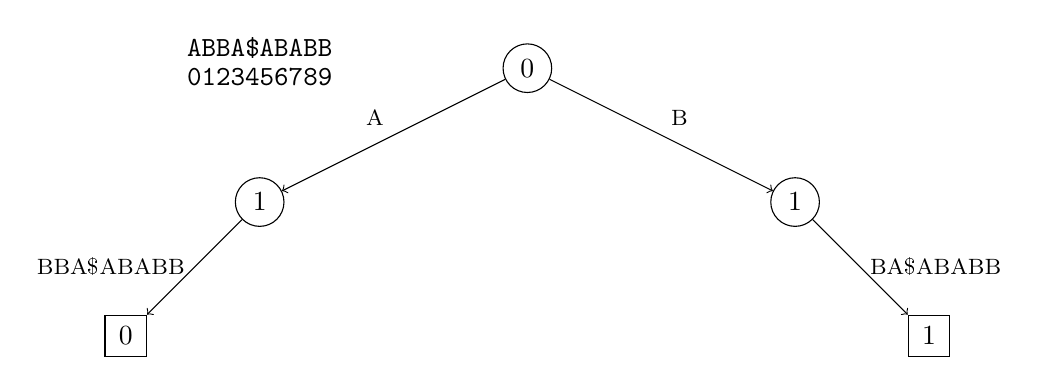
\begin{tikzpicture}[scale=1.7]
\draw (-2,0) node[above] {\texttt{A\textbf{BBA\$ABABB}}};
\draw (-2,-0.2) node[above] {\texttt{0123456789}};
\path (0,0) node[circle,minimum size=15pt,draw] (00) {0};

\path (-2,-1) node[circle,minimum size=15pt,draw] (A){1};
\draw[->] (00) -- node[above left]{\footnotesize A} (A);
\path (-3,-2) node[rectangle,minimum size=15pt,draw] (AB){0};
\draw[->] (A) -- node[left]{\footnotesize BBA\$ABABB} (AB);

\path (2,-1) node[circle,minimum size=15pt,draw] (B){1};
\draw[->] (00) -- node[above right]{\footnotesize B} (B);
\path (3,-2) node[rectangle,minimum size=15pt,draw] (BB){1};
\draw[->] (B) -- node[right]{\footnotesize BA\$ABABB} (BB);
\end{tikzpicture}}

\only<3>{\hspace*{-0.25cm}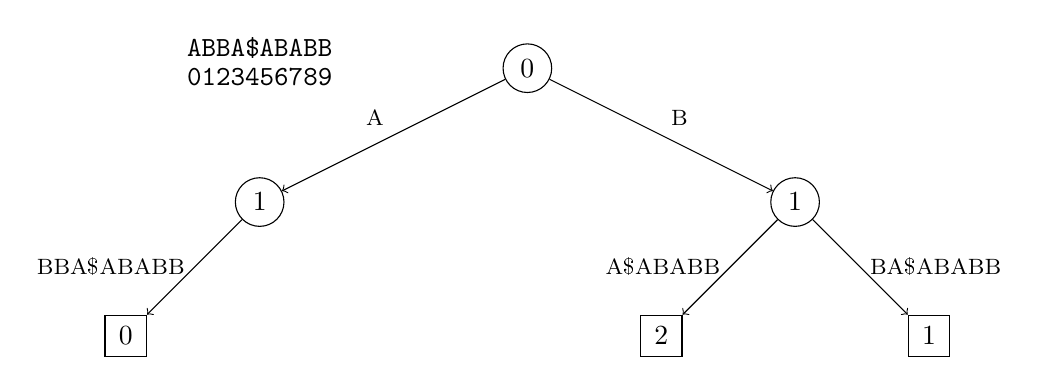
\begin{tikzpicture}[scale=1.7]
\draw (-2,0) node[above] {\texttt{AB\textbf{BA\$ABABB}}};
\draw (-2,-0.2) node[above] {\texttt{0123456789}};
\path (0,0) node[circle,minimum size=15pt,draw] (00) {0};

\path (-2,-1) node[circle,minimum size=15pt,draw] (A){1};
\draw[->] (00) -- node[above left]{\footnotesize A} (A);
\path (-3,-2) node[rectangle,minimum size=15pt,draw] (AB){0};
\draw[->] (A) -- node[left]{\footnotesize BBA\$ABABB} (AB);

\path (2,-1) node[circle,minimum size=15pt,draw] (B){1};
\draw[->] (00) -- node[above right]{\footnotesize B} (B);
\path (3,-2) node[rectangle,minimum size=15pt,draw] (BB){1};
\draw[->] (B) -- node[right]{\footnotesize BA\$ABABB} (BB);

\path (1,-2) node[rectangle,minimum size=15pt,draw] (BA){2};
\draw[->] (B) -- node[left]{\footnotesize A\$ABABB} (BA);
\end{tikzpicture}}

\only<4>{\hspace*{-0.25cm}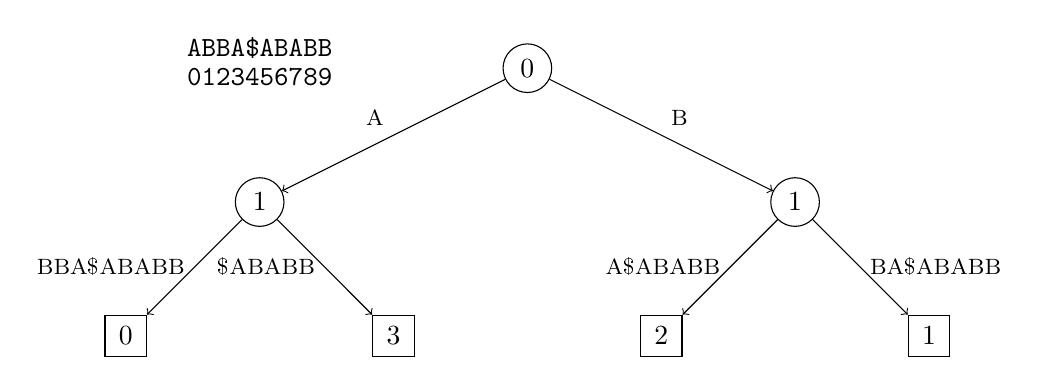
\begin{tikzpicture}[scale=1.7]
\draw (-2,0) node[above] {\texttt{ABB\textbf{A\$ABABB}}};
\draw (-2,-0.2) node[above] {\texttt{0123456789}};
\path (0,0) node[circle,minimum size=15pt,draw] (00) {0};

\path (-2,-1) node[circle,minimum size=15pt,draw] (A){1};
\draw[->] (00) -- node[above left]{\footnotesize A} (A);
\path (-3,-2) node[rectangle,minimum size=15pt,draw] (AB){0};
\draw[->] (A) -- node[left]{\footnotesize BBA\$ABABB} (AB);

\path (2,-1) node[circle,minimum size=15pt,draw] (B){1};
\draw[->] (00) -- node[above right]{\footnotesize B} (B);
\path (3,-2) node[rectangle,minimum size=15pt,draw] (BB){1};
\draw[->] (B) -- node[right]{\footnotesize BA\$ABABB} (BB);

\path (1,-2) node[rectangle,minimum size=15pt,draw] (BA){2};
\draw[->] (B) -- node[left]{\footnotesize A\$ABABB} (BA);

\path (-1,-2) node[rectangle,minimum size=15pt,draw] (AS){3};
\draw[->] (A) -- node[left]{\footnotesize \$ABABB} (AS);
\end{tikzpicture}}

\only<5>{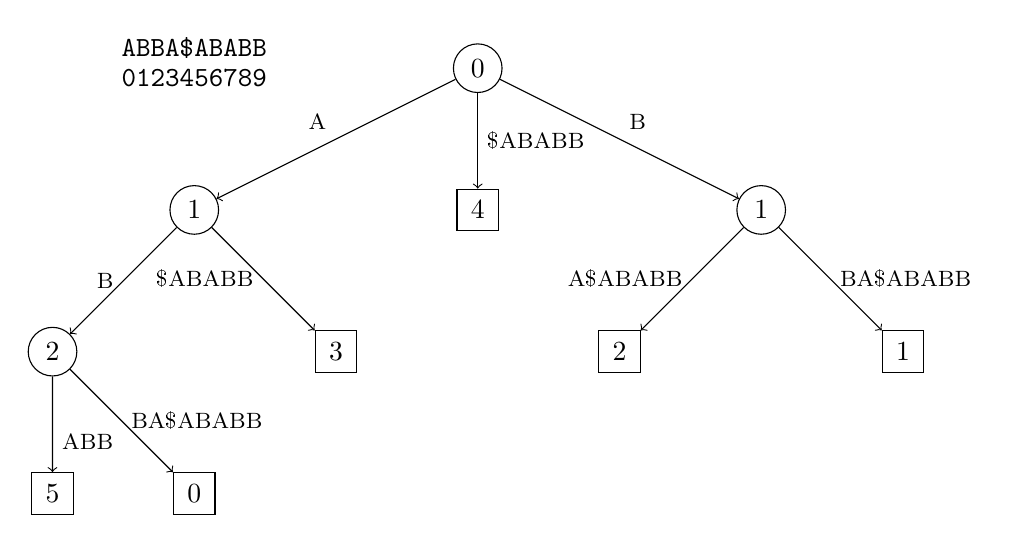
\begin{tikzpicture}[scale=1.8]
\draw (-2,0) node[above] {\texttt{ABBA\$\textbf{ABABB}}};
\draw (-2,-0.2) node[above] {\texttt{0123456789}};
\path (0,0) node[circle,minimum size=15pt,draw] (00) {0};

\path (-2,-1) node[circle,minimum size=15pt,draw] (A){1};
\draw[->] (00) -- node[above left]{\footnotesize A} (A);
\path (-3,-2) node[circle,minimum size=15pt,draw] (AB){2};
\draw[->] (A) -- node[left]{\footnotesize B} (AB);

\path (2,-1) node[circle,minimum size=15pt,draw] (B){1};
\draw[->] (00) -- node[above right]{\footnotesize B} (B);
\path (3,-2) node[rectangle,minimum size=15pt,draw] (BB){1};
\draw[->] (B) -- node[right]{\footnotesize BA\$ABABB} (BB);

\path (1,-2) node[rectangle,minimum size=15pt,draw] (BA){2};
\draw[->] (B) -- node[left]{\footnotesize A\$ABABB} (BA);

\path (-1,-2) node[rectangle,minimum size=15pt,draw] (AS){3};
\draw[->] (A) -- node[left]{\footnotesize \$ABABB} (AS);

\path (-2,-3) node[rectangle,minimum size=15pt,draw] (ABB){0};
\draw[->] (AB) -- node[right]{\footnotesize BA\$ABABB} (ABB);
\path (-3,-3) node[rectangle,minimum size=15pt,draw] (ABB0){5};
\draw[->] (AB) -- node[below right]{\footnotesize ABB} (ABB0);

\path (0,-1) node[rectangle,minimum size=15pt,draw] (S){4};
\draw[->] (00) -- node[right]{\footnotesize \$ABABB} (S);
\end{tikzpicture}}

\only<6>{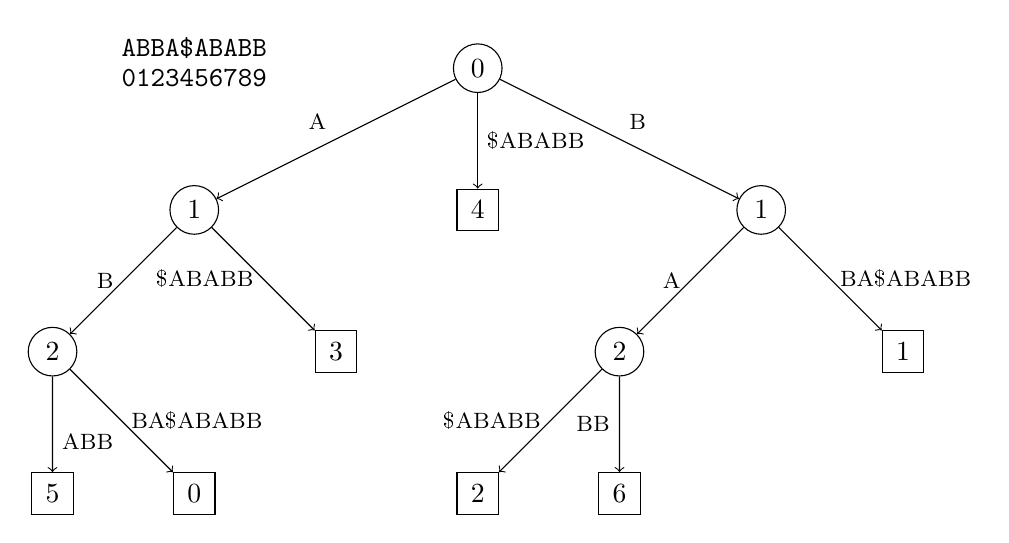
\begin{tikzpicture}[scale=1.8]
\draw (-2,0) node[above] {\texttt{ABBA\$A\textbf{BABB}}};
\draw (-2,-0.2) node[above] {\texttt{0123456789}};
\path (0,0) node[circle,minimum size=15pt,draw] (00) {0};

\path (-2,-1) node[circle,minimum size=15pt,draw] (A){1};
\draw[->] (00) -- node[above left]{\footnotesize A} (A);
\path (-3,-2) node[circle,minimum size=15pt,draw] (AB){2};
\draw[->] (A) -- node[left]{\footnotesize B} (AB);

\path (2,-1) node[circle,minimum size=15pt,draw] (B){1};
\draw[->] (00) -- node[above right]{\footnotesize B} (B);
\path (3,-2) node[rectangle,minimum size=15pt,draw] (BB){1};
\draw[->] (B) -- node[right]{\footnotesize BA\$ABABB} (BB);

\path (1,-2) node[circle,minimum size=15pt,draw] (BA){2};
\draw[->] (B) -- node[left]{\footnotesize A} (BA);

\path (-1,-2) node[rectangle,minimum size=15pt,draw] (AS){3};
\draw[->] (A) -- node[left]{\footnotesize \$ABABB} (AS);

\path (-2,-3) node[rectangle,minimum size=15pt,draw] (ABB){0};
\draw[->] (AB) -- node[right]{\footnotesize BA\$ABABB} (ABB);
\path (-3,-3) node[rectangle,minimum size=15pt,draw] (ABB0){5};
\draw[->] (AB) -- node[below right]{\footnotesize ABB} (ABB0);

\path (0,-3) node[rectangle,minimum size=15pt,draw] (BAS){2};
\draw[->] (BA) -- node[left]{\footnotesize \$ABABB} (BAS);
\path (1,-3) node[rectangle,minimum size=15pt,draw] (BAB){6};
\draw[->] (BA) -- node[left]{\footnotesize BB} (BAB);

\path (0,-1) node[rectangle,minimum size=15pt,draw] (S){4};
\draw[->] (00) -- node[right]{\footnotesize \$ABABB} (S);
\end{tikzpicture}}

\only<7>{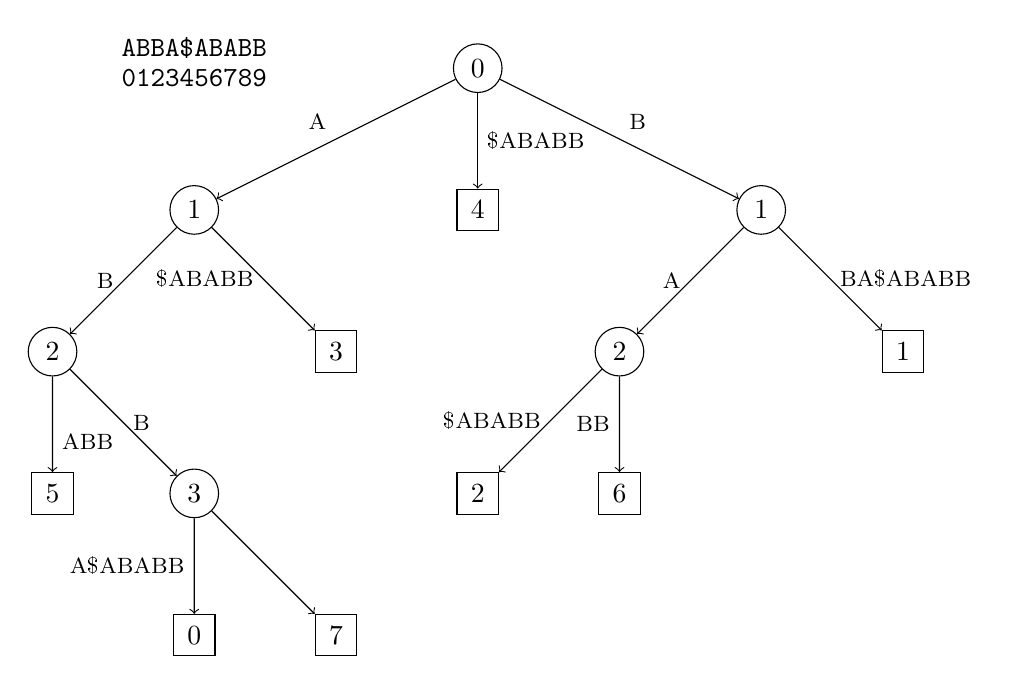
\begin{tikzpicture}[scale=1.8]
\draw (-2,0) node[above] {\texttt{ABBA\$AB\textbf{ABB}}};
\draw (-2,-0.2) node[above] {\texttt{0123456789}};
\path (0,0) node[circle,minimum size=15pt,draw] (00) {0};

\path (-2,-1) node[circle,minimum size=15pt,draw] (A){1};
\draw[->] (00) -- node[above left]{\footnotesize A} (A);
\path (-3,-2) node[circle,minimum size=15pt,draw] (AB){2};
\draw[->] (A) -- node[left]{\footnotesize B} (AB);

\path (2,-1) node[circle,minimum size=15pt,draw] (B){1};
\draw[->] (00) -- node[above right]{\footnotesize B} (B);
\path (3,-2) node[rectangle,minimum size=15pt,draw] (BB){1};
\draw[->] (B) -- node[right]{\footnotesize BA\$ABABB} (BB);

\path (1,-2) node[circle,minimum size=15pt,draw] (BA){2};
\draw[->] (B) -- node[left]{\footnotesize A} (BA);

\path (-1,-2) node[rectangle,minimum size=15pt,draw] (AS){3};
\draw[->] (A) -- node[left]{\footnotesize \$ABABB} (AS);

\path (-2,-3) node[circle,minimum size=15pt,draw] (ABB){3};
\draw[->] (AB) -- node[right]{\footnotesize B} (ABB);
\path (-3,-3) node[rectangle,minimum size=15pt,draw] (ABB0){5};
\draw[->] (AB) -- node[below right]{\footnotesize ABB} (ABB0);

\path (0,-3) node[rectangle,minimum size=15pt,draw] (BAS){2};
\draw[->] (BA) -- node[left]{\footnotesize \$ABABB} (BAS);
\path (1,-3) node[rectangle,minimum size=15pt,draw] (BAB){6};
\draw[->] (BA) -- node[left]{\footnotesize BB} (BAB);

\path (-2,-4) node[rectangle,minimum size=15pt,draw] (ABBA){0};
\draw[->] (ABB) -- node[left]{\footnotesize A\$ABABB} (ABBA);
\path (-1,-4) node[rectangle,minimum size=15pt,draw] (BAB0){7};
\draw[->] (ABB) -- node[left]{ } (BAB0);

\path (0,-1) node[rectangle,minimum size=15pt,draw] (S){4};
\draw[->] (00) -- node[right]{\footnotesize \$ABABB} (S);
\end{tikzpicture}}

\only<8>{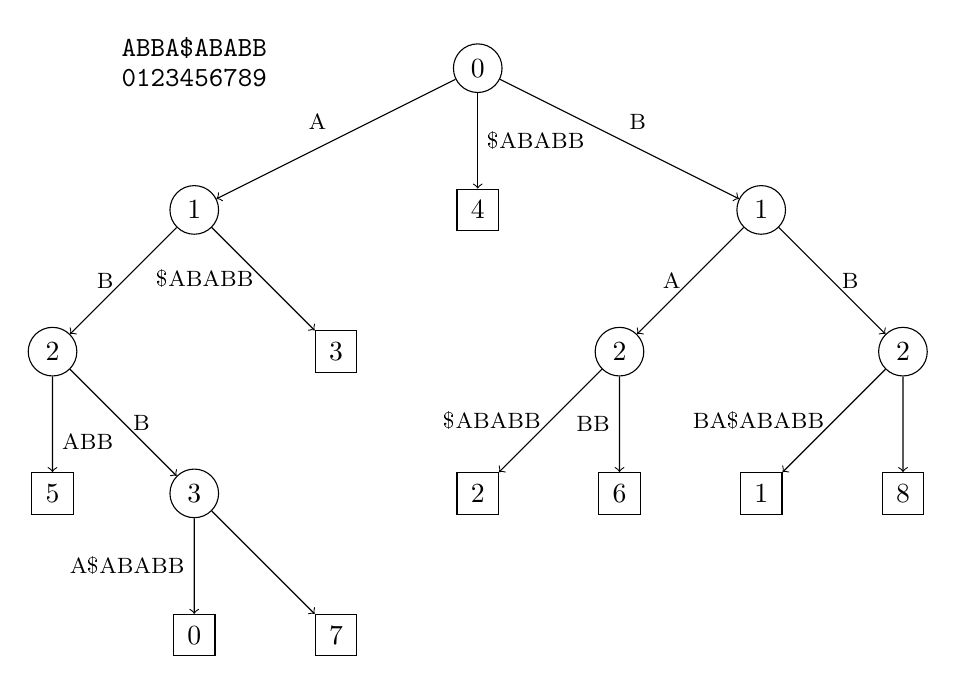
\begin{tikzpicture}[scale=1.8]
\draw (-2,0) node[above] {\texttt{ABBA\$ABA\textbf{BB}}};
\draw (-2,-0.2) node[above] {\texttt{0123456789}};
\path (0,0) node[circle,minimum size=15pt,draw] (00) {0};

\path (-2,-1) node[circle,minimum size=15pt,draw] (A){1};
\draw[->] (00) -- node[above left]{\footnotesize A} (A);
\path (-3,-2) node[circle,minimum size=15pt,draw] (AB){2};
\draw[->] (A) -- node[left]{\footnotesize B} (AB);

\path (2,-1) node[circle,minimum size=15pt,draw] (B){1};
\draw[->] (00) -- node[above right]{\footnotesize B} (B);
\path (3,-2) node[circle,minimum size=15pt,draw] (BB){2};
\draw[->] (B) -- node[right]{\footnotesize B} (BB);

\path (1,-2) node[circle,minimum size=15pt,draw] (BA){2};
\draw[->] (B) -- node[left]{\footnotesize A} (BA);

\path (-1,-2) node[rectangle,minimum size=15pt,draw] (AS){3};
\draw[->] (A) -- node[left]{\footnotesize \$ABABB} (AS);

\path (-2,-3) node[circle,minimum size=15pt,draw] (ABB){3};
\draw[->] (AB) -- node[right]{\footnotesize B} (ABB);
\path (-3,-3) node[rectangle,minimum size=15pt,draw] (ABB0){5};
\draw[->] (AB) -- node[below right]{\footnotesize ABB} (ABB0);

\path (0,-3) node[rectangle,minimum size=15pt,draw] (BAS){2};
\draw[->] (BA) -- node[left]{\footnotesize \$ABABB} (BAS);
\path (1,-3) node[rectangle,minimum size=15pt,draw] (BAB){6};
\draw[->] (BA) -- node[left]{\footnotesize BB} (BAB);

\path (-2,-4) node[rectangle,minimum size=15pt,draw] (ABBA){0};
\draw[->] (ABB) -- node[left]{\footnotesize A\$ABABB} (ABBA);
\path (-1,-4) node[rectangle,minimum size=15pt,draw] (BAB0){7};
\draw[->] (ABB) -- node[left]{ } (BAB0);

\path (3,-3) node[rectangle,minimum size=15pt,draw] (BB0){8};
\draw[->] (BB) -- node[above right]{\footnotesize } (BB0);
\path (2,-3) node[rectangle,minimum size=15pt,draw] (BBA){1};
\draw[->] (BB) -- node[left]{\footnotesize BA\$ABABB} (BBA);

\path (0,-1) node[rectangle,minimum size=15pt,draw] (S){4};
\draw[->] (00) -- node[right]{\footnotesize \$ABABB} (S);
\end{tikzpicture}}

\only<9>{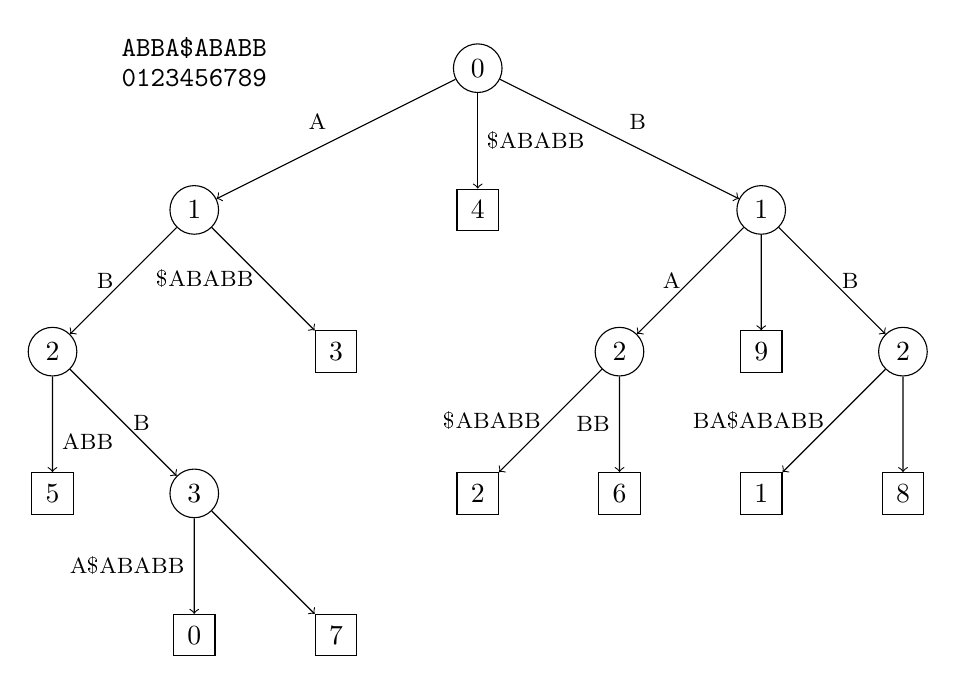
\begin{tikzpicture}[scale=1.8]
\draw (-2,0) node[above] {\texttt{ABBA\$ABAB\textbf{B}}};
\draw (-2,-0.2) node[above] {\texttt{0123456789}};
\path (0,0) node[circle,minimum size=15pt,draw] (00) {0};

\path (-2,-1) node[circle,minimum size=15pt,draw] (A){1};
\draw[->] (00) -- node[above left]{\footnotesize A} (A);
\path (-3,-2) node[circle,minimum size=15pt,draw] (AB){2};
\draw[->] (A) -- node[left]{\footnotesize B} (AB);

\path (2,-1) node[circle,minimum size=15pt,draw] (B){1};
\draw[->] (00) -- node[above right]{\footnotesize B} (B);
\path (3,-2) node[circle,minimum size=15pt,draw] (BB){2};
\draw[->] (B) -- node[right]{\footnotesize B} (BB);

\path (1,-2) node[circle,minimum size=15pt,draw] (BA){2};
\draw[->] (B) -- node[left]{\footnotesize A} (BA);

\path (-1,-2) node[rectangle,minimum size=15pt,draw] (AS){3};
\draw[->] (A) -- node[left]{\footnotesize \$ABABB} (AS);

\path (-2,-3) node[circle,minimum size=15pt,draw] (ABB){3};
\draw[->] (AB) -- node[right]{\footnotesize B} (ABB);
\path (-3,-3) node[rectangle,minimum size=15pt,draw] (ABB0){5};
\draw[->] (AB) -- node[below right]{\footnotesize ABB} (ABB0);

\path (0,-3) node[rectangle,minimum size=15pt,draw] (BAS){2};
\draw[->] (BA) -- node[left]{\footnotesize \$ABABB} (BAS);
\path (1,-3) node[rectangle,minimum size=15pt,draw] (BAB){6};
\draw[->] (BA) -- node[left]{\footnotesize BB} (BAB);

\path (-2,-4) node[rectangle,minimum size=15pt,draw] (ABBA){0};
\draw[->] (ABB) -- node[left]{\footnotesize A\$ABABB} (ABBA);
\path (-1,-4) node[rectangle,minimum size=15pt,draw] (BAB0){7};
\draw[->] (ABB) -- node[left]{ } (BAB0);

\path (3,-3) node[rectangle,minimum size=15pt,draw] (BB0){8};
\draw[->] (BB) -- node[above right]{\footnotesize } (BB0);
\path (2,-3) node[rectangle,minimum size=15pt,draw] (BBA){1};
\draw[->] (BB) -- node[left]{\footnotesize BA\$ABABB} (BBA);

\path (2,-2) node[rectangle,minimum size=15pt,draw] (B0){9};
\draw[->] (B) -- node[above right]{\footnotesize } (B0);

\path (0,-1) node[rectangle,minimum size=15pt,draw] (S){4};
\draw[->] (00) -- node[right]{\footnotesize \$ABABB} (S);
\end{tikzpicture}}
\end{frame}

\begin{frame}{Finding MUMs from suffix tree}
Let's recall what condition MUMs had to have:
\begin{enumerate}
\item Exact matches on both genomes.
\item Surrounded by mismatches.
\item Unique.
\end{enumerate}
We can achieve conditions 1 and 3 by searching the tree for a internal with exactly two leafs which have to start on each side of the dollar sign (on each genome).

\vspace*{0.1cm}
We'll need to check for condition 2 separately.

\end{frame}

\begin{frame}{Finding potential MUMs}
\only<1>{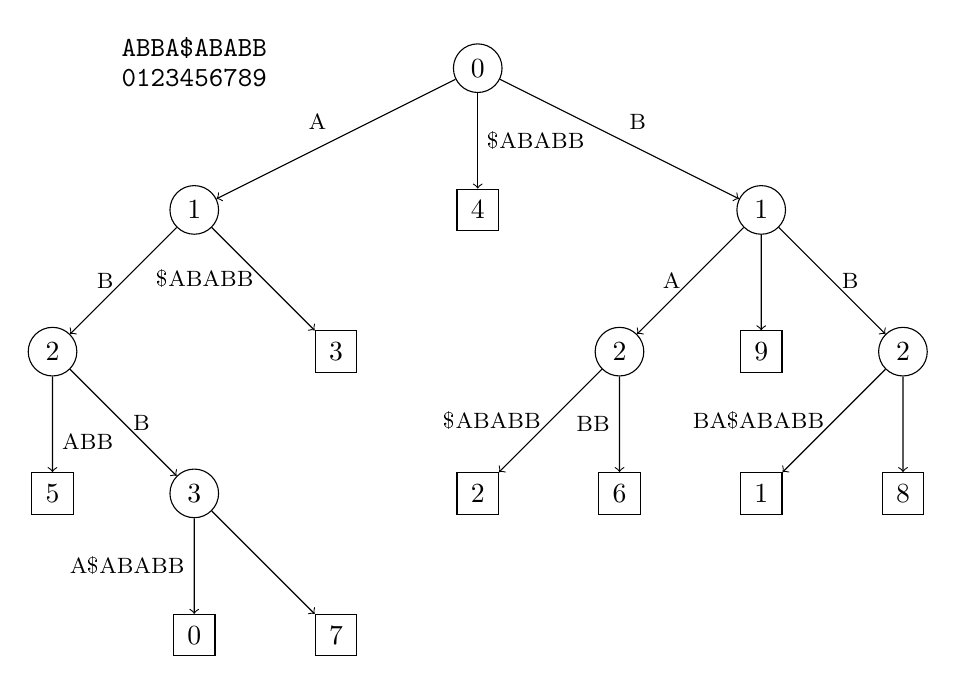
\begin{tikzpicture}[scale=1.8]
\draw (-2,0) node[above] {\texttt{ABBA\$ABABB}};
\draw (-2,-0.2) node[above] {\texttt{0123456789}};
\path (0,0) node[circle,minimum size=15pt,draw] (00) {0};

\path (-2,-1) node[circle,minimum size=15pt,draw] (A){1};
\draw[->] (00) -- node[above left]{\footnotesize A} (A);
\path (-3,-2) node[circle,minimum size=15pt,draw] (AB){2};
\draw[->] (A) -- node[left]{\footnotesize B} (AB);

\path (2,-1) node[circle,minimum size=15pt,draw] (B){1};
\draw[->] (00) -- node[above right]{\footnotesize B} (B);
\path (3,-2) node[circle,minimum size=15pt,draw] (BB){2};
\draw[->] (B) -- node[right]{\footnotesize B} (BB);

\path (1,-2) node[circle,minimum size=15pt,draw] (BA){2};
\draw[->] (B) -- node[left]{\footnotesize A} (BA);

\path (-1,-2) node[rectangle,minimum size=15pt,draw] (AS){3};
\draw[->] (A) -- node[left]{\footnotesize \$ABABB} (AS);

\path (-2,-3) node[circle,minimum size=15pt,draw] (ABB){3};
\draw[->] (AB) -- node[right]{\footnotesize B} (ABB);
\path (-3,-3) node[rectangle,minimum size=15pt,draw] (ABB0){5};
\draw[->] (AB) -- node[below right]{\footnotesize ABB} (ABB0);

\path (0,-3) node[rectangle,minimum size=15pt,draw] (BAS){2};
\draw[->] (BA) -- node[left]{\footnotesize \$ABABB} (BAS);
\path (1,-3) node[rectangle,minimum size=15pt,draw] (BAB){6};
\draw[->] (BA) -- node[left]{\footnotesize BB} (BAB);

\path (-2,-4) node[rectangle,minimum size=15pt,draw] (ABBA){0};
\draw[->] (ABB) -- node[left]{\footnotesize A\$ABABB} (ABBA);
\path (-1,-4) node[rectangle,minimum size=15pt,draw] (BAB0){7};
\draw[->] (ABB) -- node[left]{ } (BAB0);

\path (3,-3) node[rectangle,minimum size=15pt,draw] (BB0){8};
\draw[->] (BB) -- node[above right]{\footnotesize } (BB0);
\path (2,-3) node[rectangle,minimum size=15pt,draw] (BBA){1};
\draw[->] (BB) -- node[left]{\footnotesize BA\$ABABB} (BBA);

\path (2,-2) node[rectangle,minimum size=15pt,draw] (B0){9};
\draw[->] (B) -- node[above right]{\footnotesize } (B0);

\path (0,-1) node[rectangle,minimum size=15pt,draw] (S){4};
\draw[->] (00) -- node[right]{\footnotesize \$ABABB} (S);
\end{tikzpicture}}

\only<2>{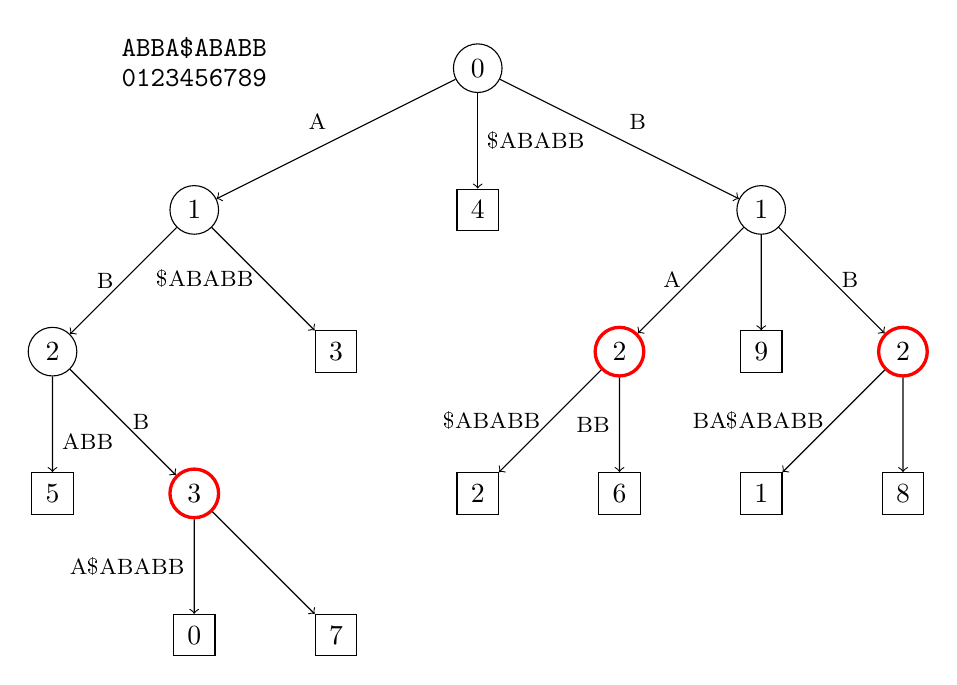
\begin{tikzpicture}[scale=1.8]
\draw (-2,0) node[above] {\texttt{ABBA\$ABABB}};
\draw (-2,-0.2) node[above] {\texttt{0123456789}};
\path (0,0) node[circle,minimum size=15pt,draw] (00) {0};

\path (-2,-1) node[circle,minimum size=15pt,draw] (A){1};
\draw[->] (00) -- node[above left]{\footnotesize A} (A);
\path (-3,-2) node[circle,minimum size=15pt,draw] (AB){2};
\draw[->] (A) -- node[left]{\footnotesize B} (AB);

\path (2,-1) node[circle,minimum size=15pt,draw] (B){1};
\draw[->] (00) -- node[above right]{\footnotesize B} (B);
\path (3,-2) node[circle,minimum size=15pt,draw=red,very thick] (BB){2};
\draw[->] (B) -- node[right]{\footnotesize B} (BB);

\path (1,-2) node[circle,minimum size=15pt,draw=red,very thick] (BA){2};
\draw[->] (B) -- node[left]{\footnotesize A} (BA);

\path (-1,-2) node[rectangle,minimum size=15pt,draw] (AS){3};
\draw[->] (A) -- node[left]{\footnotesize \$ABABB} (AS);

\path (-2,-3) node[circle,minimum size=15pt,draw=red,very thick] (ABB){3};
\draw[->] (AB) -- node[right]{\footnotesize B} (ABB);
\path (-3,-3) node[rectangle,minimum size=15pt,draw] (ABB0){5};
\draw[->] (AB) -- node[below right]{\footnotesize ABB} (ABB0);

\path (0,-3) node[rectangle,minimum size=15pt,draw] (BAS){2};
\draw[->] (BA) -- node[left]{\footnotesize \$ABABB} (BAS);
\path (1,-3) node[rectangle,minimum size=15pt,draw] (BAB){6};
\draw[->] (BA) -- node[left]{\footnotesize BB} (BAB);

\path (-2,-4) node[rectangle,minimum size=15pt,draw] (ABBA){0};
\draw[->] (ABB) -- node[left]{\footnotesize A\$ABABB} (ABBA);
\path (-1,-4) node[rectangle,minimum size=15pt,draw] (BAB0){7};
\draw[->] (ABB) -- node[left]{ } (BAB0);

\path (3,-3) node[rectangle,minimum size=15pt,draw] (BB0){8};
\draw[->] (BB) -- node[above right]{\footnotesize } (BB0);
\path (2,-3) node[rectangle,minimum size=15pt,draw] (BBA){1};
\draw[->] (BB) -- node[left]{\footnotesize BA\$ABABB} (BBA);

\path (2,-2) node[rectangle,minimum size=15pt,draw] (B0){9};
\draw[->] (B) -- node[above right]{\footnotesize } (B0);

\path (0,-1) node[rectangle,minimum size=15pt,draw] (S){4};
\draw[->] (00) -- node[right]{\footnotesize \$ABABB} (S);
\end{tikzpicture}}
\end{frame}

\begin{frame}{Potential MUMs to MUMs}
We have the following potential MUMs:
\begin{itemize}
\item \texttt{ABB} at starting positions 0 and 7.
\item \texttt{BA} at starting positions 2 and 6.
\item \texttt{BB} at starting positions 1 and 8.
\end{itemize}
Our string: \texttt{ABBA\$ABABB}
\begin{itemize}
\item \texttt{ABB} achieves condition 2 (it's surrounded by mismatches).
\item \texttt{BA} achieves condition 2 as well.
\item \texttt{BB} does NOT achieve condition 2. In both cases it is preceded by a \texttt{A}.
\end{itemize}
Resulting MUMs: \texttt{\textbf{ABB}} and \texttt{\textbf{BA}}.
\end{frame}


\begin{frame}{Results of using MUMmer}
MUMmer was put to the test on various genomes:
\begin{itemize}
\item<1-> Two strains of tuberculosis (bacteria) that are >99\% identical
\begin{itemize}
\item<1-> 5 seconds to create the suffix tree.
\item<1-> 45 seconds to sort the MUMs.
\item<1-> 5 seconds to generate the Smith-Waterman alignments of the gaps.
\end{itemize}
\item<2-> Two 'cousin' genomes. Genome of \textit{M.genitalium} (580,074 nucleotides) and \textit{M.pneumoniae} (816,394 nucleotides)
\begin{itemize}
\item<2-> 6.5 seconds to create the suffix tree.
\item<2-> 0.02 seconds to sort the MUMs.
\item<2-> 116 seconds to generate the Smith-Waterman alignments of the gaps.
\end{itemize}
\item<3-> Subsequence of a human chromosome 12p13 and mouse chromosome 6 (both rougly 230,000 nucleotides)
\begin{itemize}
\item<3-> 1.6 seconds to create the suffix tree.
\item<3-> $\approx$ 0 seconds to sort the MUMs.
\item<3-> 27.4 seconds to generate the Smith-Waterman alignments of the gaps.
\end{itemize}
\end{itemize}

\end{frame}

\begin{frame}{MUMmer 3}
\begin{itemize}
\item MUMmer 3 is the latest version of MUMmer
\item It was released in 2004 and is open-source.
\item Requires less than half the memory and more than twice as fast than the initial MUMmer.
\item Most notable problems fixed and options added since the initial MUMmer:
\begin{itemize}
\item You can allow tolarence for mismatches when finding MUMs.
\item Can handle MUMs that are not necessarily unique.
\item All sorts of visualization tools.
\end{itemize}
\item Could successfully compare all human chromosomes to each other. Tests were performed on a single computer with 950 MHz processor.
\begin{itemize}
\item Computation time: 4.5 days
\item Memory used: 3.9 GB
\end{itemize}
\end{itemize}
\end{frame}



\end{document}
